\documentclass{article}

% Language setting
% Replace `english' with e.g. `spanish' to change the document language
\usepackage[english]{babel}

% Set page size and margins
% Replace `letterpaper' with `a4paper' for UK/EU standard size
\usepackage[letterpaper,top=2cm,bottom=2cm,left=2cm,right=2cm,marginparwidth=1.75cm]{geometry}

% Useful packages
\usepackage{amsmath}
\usepackage{mathtools}
\usepackage{graphicx}
\usepackage{array}
\usepackage[colorlinks=true, allcolors=blue]{hyperref}
\usepackage{matlab-prettifier}

\usepackage{amssymb}
\usepackage{algorithm}
\usepackage{float}  % Figure placement
\usepackage{minted}  % Code highlighting
\usepackage{tikz}  % Flow chart
\usepackage{lipsum}
\usepackage{xspace}
\usepackage{hyperref}
\usepackage{MnSymbol}
\usepackage{pgffor}
\usepackage{indentfirst}
\usepackage{colortbl}
\usepackage{multirow}
\usepackage{array}
\usepackage{mdframed}
\usepackage{enumitem}

\usepackage{listings}

\usepackage{tabularx}


\usetikzlibrary{positioning} % Added by TQBH
\usetikzlibrary {graphs} % Added by TQBH
\usetikzlibrary {graphs.standard} % Added by TQBH

\newcommand{\abs}[1]{\left\lvert #1 \right\rvert}

\title{CSCI598B - Robot Mapping (SLAM)\\
Project Report}
\author{Group 6: \\ 
Farid Boulos, Keenan Buckley, Randi Higashi,\\ 
Bill Huynh, Priestly Barigala, Aarushi Doctor}
\date{April 30, 2024}


\begin{document}
\maketitle

\section*{I - Homework 04}

\section*{1 - Exercise 1}

\section*{a) Step 1}

Downsampling is done by using the Open3D VoxelDownSample() function on each point cloud (Voxel Grid downsampling).

For RGBD data: \autoref{fig:pc0-rgbd-down} shows downsampling effects compared to \autoref{fig:pc0-rgbd-org}, with voxel size parameter 0.05.

For LiDAR data: \autoref{fig:pc0-lidar-down} shows downsampling effects compared to \autoref{fig:pc0-lidar-org}, with voxel size parameter 0.4.

\begin{figure}[H]
    \centering
    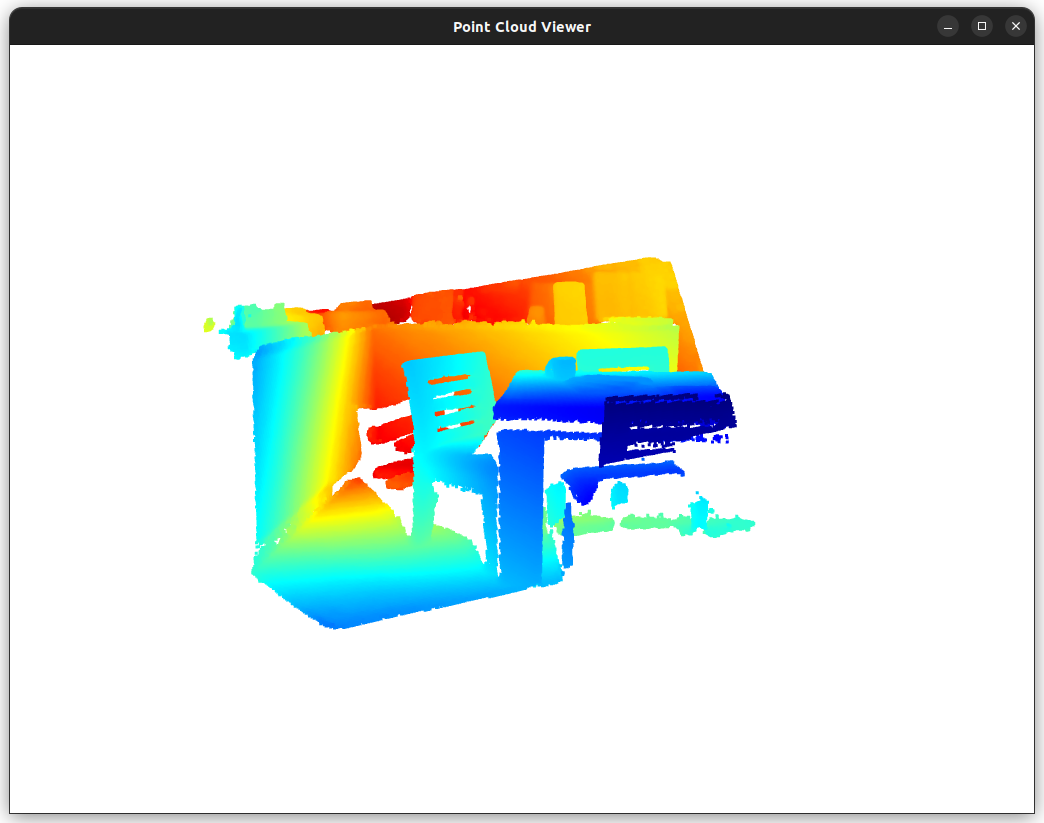
\includegraphics[width=0.7\linewidth]{pc0-rgbd-org.png}
    \caption{\label{fig:pc0-rgbd-org}Snapshot of RGBD point cloud index 0 before downsampling.}
\end{figure}

\begin{figure}[H]
    \centering
    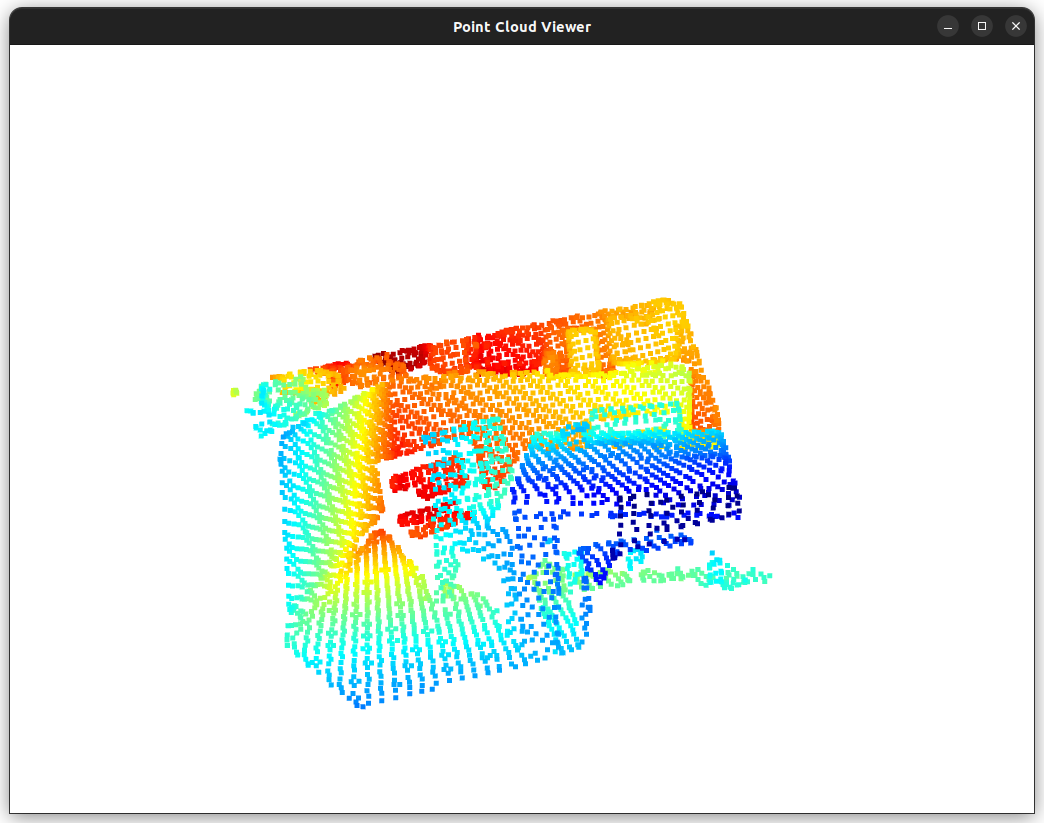
\includegraphics[width=0.7\linewidth]{pc0-rgbd-down.png}
    \caption{\label{fig:pc0-rgbd-down}Snapshot of RGBD point cloud index 0 after downsampling.}
\end{figure}

\begin{figure}[H]
    \centering
    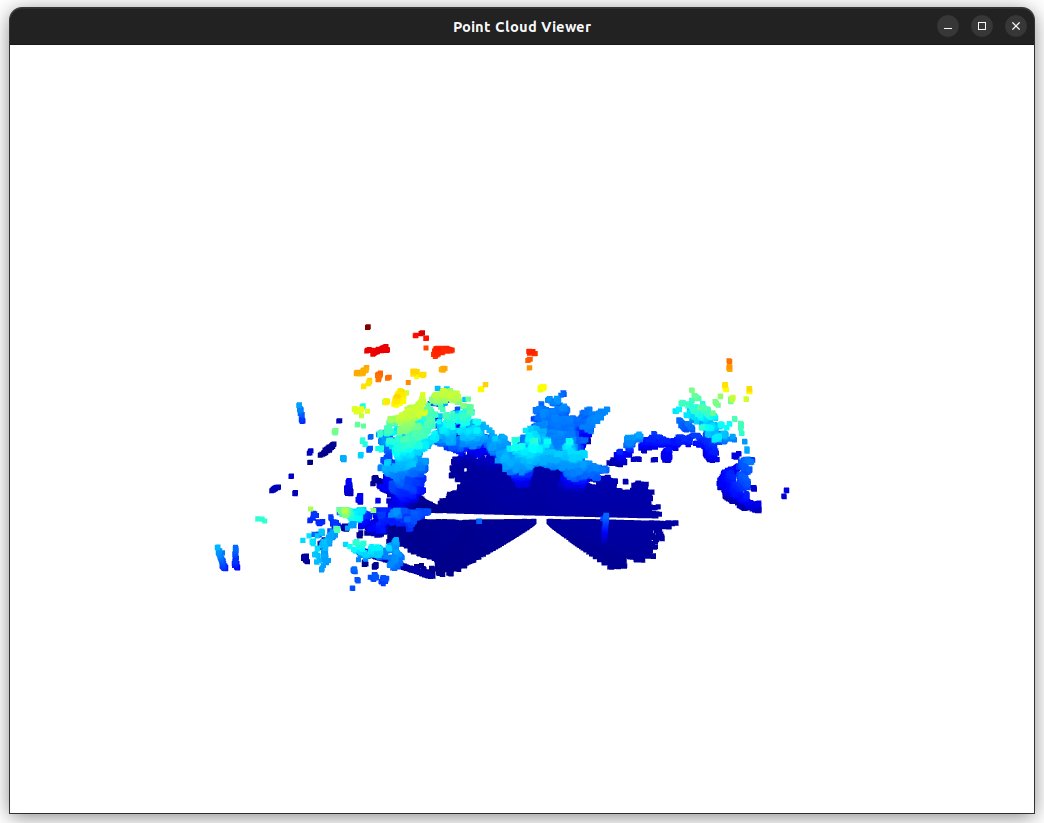
\includegraphics[width=0.7\linewidth]{pc0-lidar-org.png}
    \caption{\label{fig:pc0-lidar-org}Snapshot of LiDAR point cloud index 0 before downsampling.}
\end{figure}

\begin{figure}[H]
    \centering
    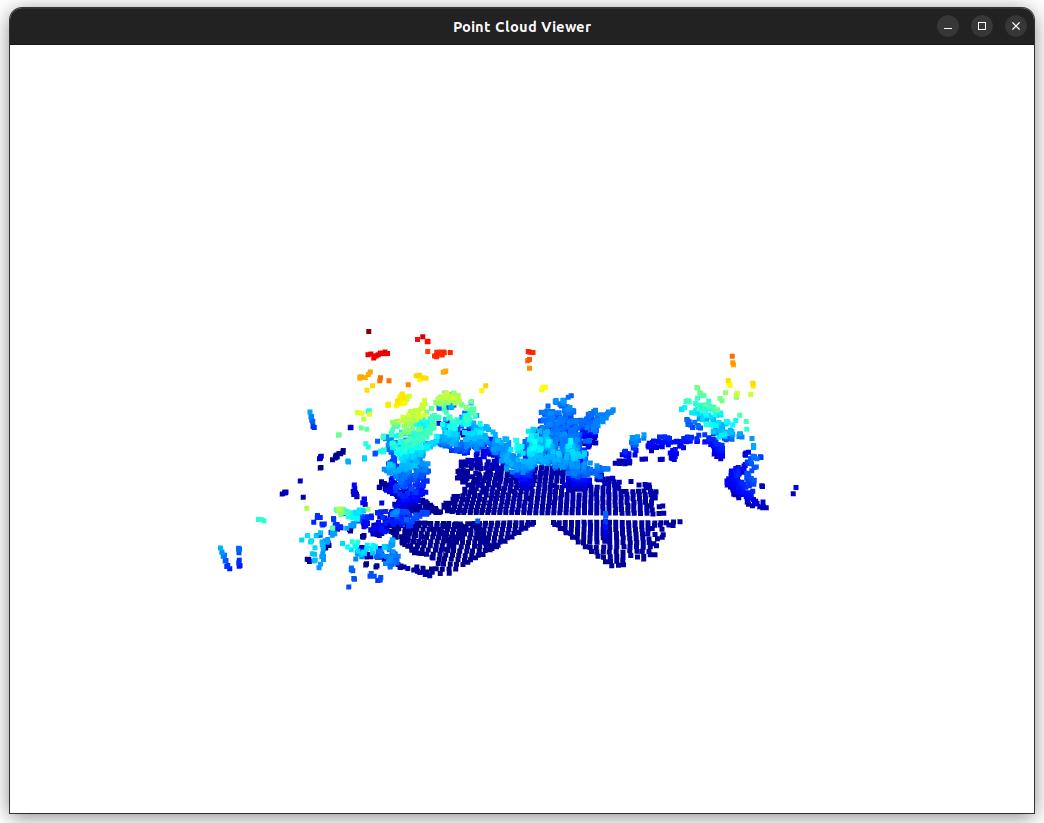
\includegraphics[width=0.7\linewidth]{pc0-lidar-down.png}
    \caption{\label{fig:pc0-lidar-down}Snapshot of LiDAR point cloud index 0 after downsampling.}
\end{figure}


\section*{b) Step 2-3}

ICP on RGBD data:
\begin{itemize}
    \item Registration result returned by ICP: a transformation matrix (shown here is to transform from point cloud index 0 to point cloud index 1):
        \begin{flalign*}
            \begin{bmatrix}
                0.997235 & -0.0639747 & 0.0378039 & 0.114175\\
                0.0647506 & 0.997708 & -0.0196679 & 0.057978 \\
                -0.0364589 & 0.0220614 & 0.999092 & -0.126685 \\
                0 & 0 & 0 & 1
            \end{bmatrix}
        \end{flalign*}
    \item Result fusion of all point clouds:
        \begin{figure}[H]
            \centering
            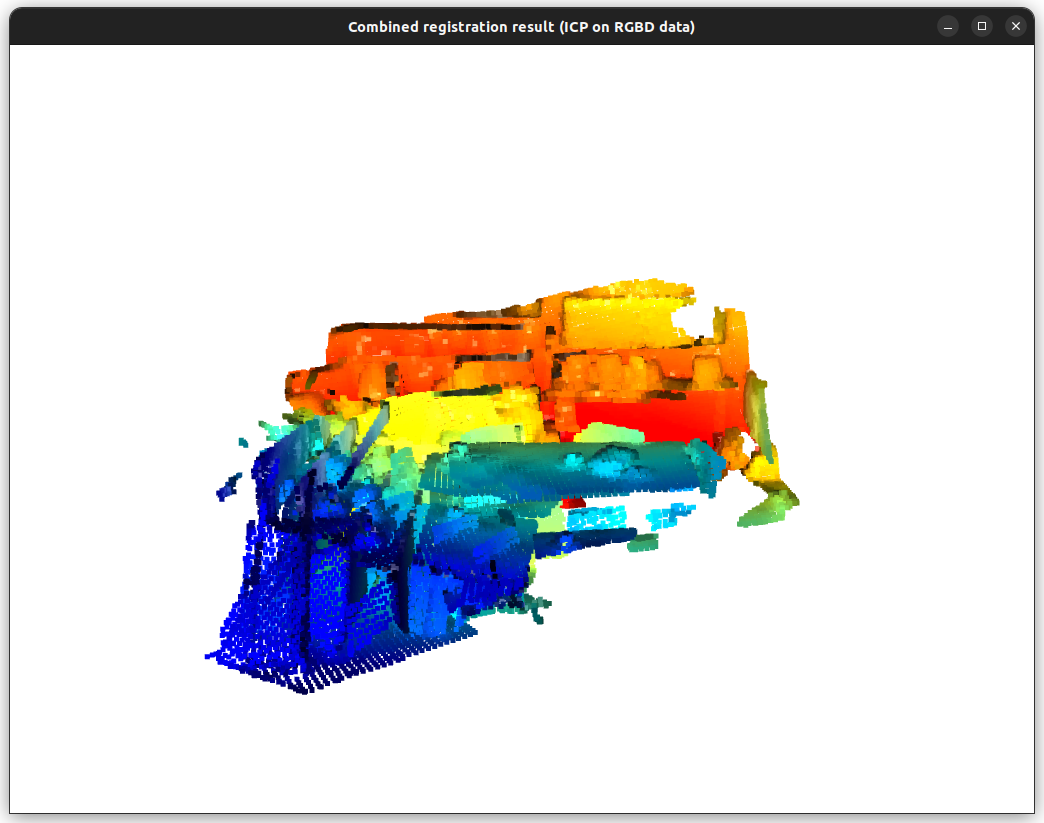
\includegraphics[width=0.7\linewidth]{ICP-on-RGBD-3.png}
            \caption{\label{fig:ICP-on-RGBD-3}Result fused point clouds, using ICP on RGBD data.}
        \end{figure}
    \item Judging from gradually registering the point clouds, ICP performs reasonably with the first 3 point clouds (indices 0 to 2). It starts showing inaccurate registration results from point clouds of index 3 on. \textbf{Overall, ICP failed to show an adequate registration result for all RGBD point clouds.}
\end{itemize}

\hspace{1cm}

RANSAC on RGBD data:
\begin{itemize}
    \item Registration result returned by RANSAC: a transformation matrix (shown here is to transform from point cloud index 0 to point cloud index 1):
        \begin{flalign*}
            \begin{bmatrix}
                0.99583 & -0.0709411 & 0.057351 & 0.0591225\\
                0.0714476 & 0.997421 & -0.00682798 & 0.0265614 \\
                -0.0567187 & 0.0108971 & 0.998331 & -0.121719 \\
                0 & 0 & 0 & 1
            \end{bmatrix}
        \end{flalign*}
    \item FPFH features are obtained using the ComputeFPFHFeature() function in Open3D. We need FPFH features for both the source and the target point clouds. To compute FPFH features, the normals of each point cloud and KD-tree search parameters are also necessary. We tried to search for ways to visualize feature points but could not find one.
    \item Result fusion of all point clouds:
        \begin{figure}[H]
            \centering
            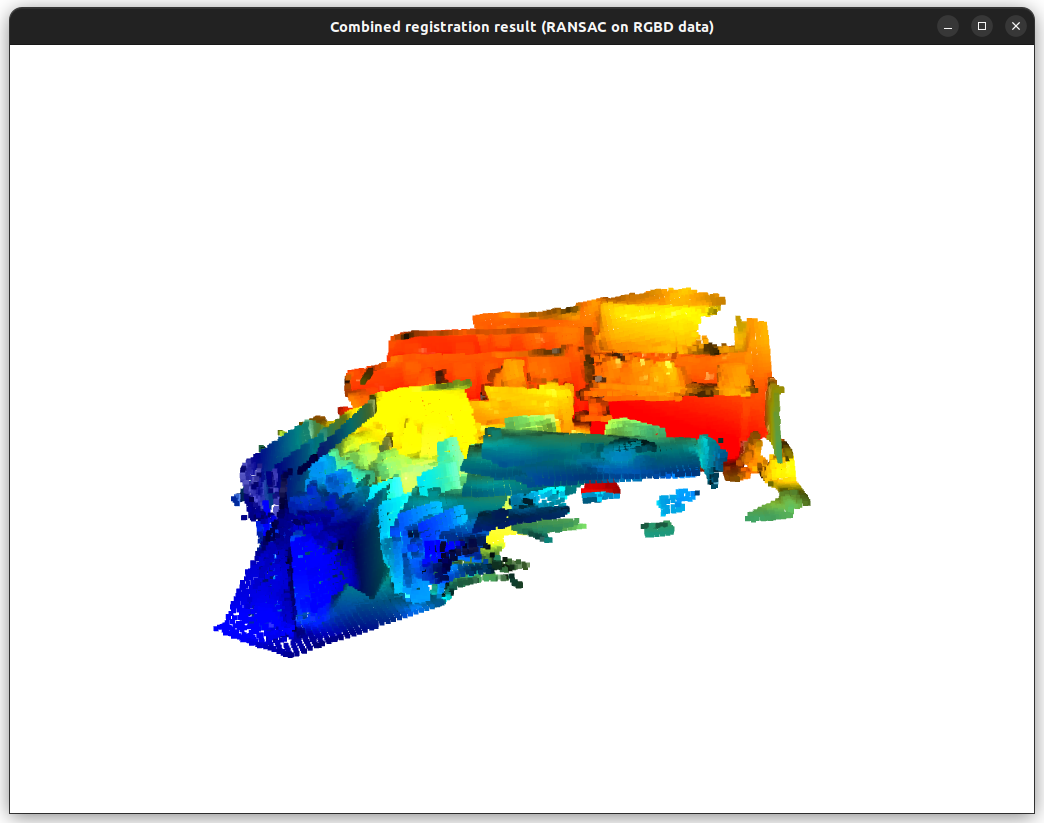
\includegraphics[width=0.7\linewidth]{RANSAC-on-RGBD-3.png}
            \caption{\label{fig:RANSAC-on-RGBD-3}Result fused point clouds, using RANSAC on RGBD data.}
        \end{figure}
    \item RANSAC performs reasonably with the first 4 point clouds (indices 0 to 3). It starts showing inaccurate registration results from point clouds of index 4 on. \textbf{Overall, RANSAC also failed to show an adequate registration result for all RGBD point clouds. However, the results are better compared to ICP on RGBD data.}
\end{itemize}

\hspace{2cm}

ICP on LiDAR data:
\begin{itemize}
    \item Registration result returned by ICP: a transformation matrix (shown here is to transform from point cloud index 0 to point cloud index 1):
        \begin{flalign*}
            \begin{bmatrix}
                0.999425 & 0.0321274 & 0.0108199 & -0.756738\\
                -0.0321099 & 0.999483 & -0.00178754 & -0.0413416 \\
                -0.0108717 & 0.00143908 & 0.99994 & -0.00956993 \\
                0 & 0 & 0 & 1
            \end{bmatrix}
        \end{flalign*}
    \item Result fusion of all point clouds:
        \begin{figure}[H]
            \centering
            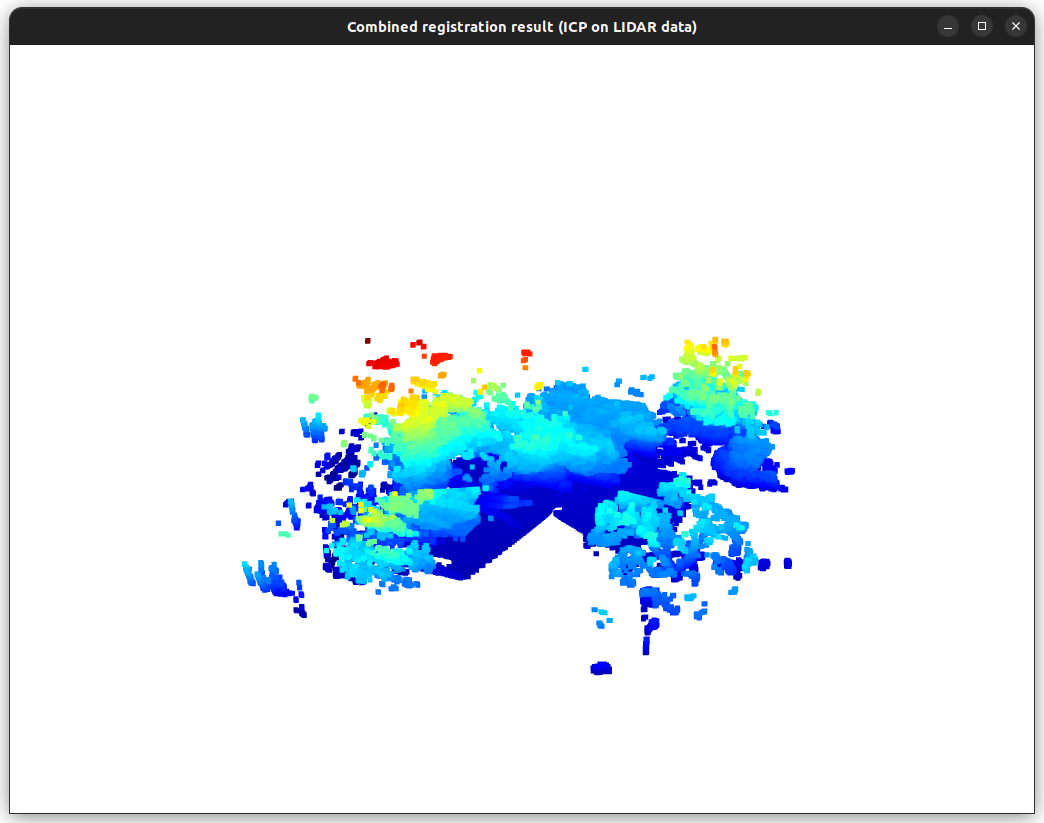
\includegraphics[width=0.7\linewidth]{ICP-on-LIDAR-3.png}
            \caption{\label{fig:ICP-on-LIDAR-3}Result fused point clouds, using ICP on LiDAR data.}
        \end{figure}
    \item Although there are still inaccuracies in the registration, the result fused point clouds show a scene with several small trees. \textbf{We can say ICP did not fail to register the LiDAR point clouds.}
\end{itemize}

\hspace{1cm}

RANSAC on LiDAR data:
\begin{itemize}
    \item Registration result returned by RANSAC: a transformation matrix (shown here is to transform from point cloud index 0 to point cloud index 1):
        \begin{flalign*}
            \begin{bmatrix}
                0.998775 & 0.0375367 & 0.0322403 & -0.902379\\
                -0.0376827 & 0.999282 & 0.0039351 & -0.105385 \\
                -0.0320694 & -0.00514518 & 0.999472 & -0.0202583 \\
                0 & 0 & 0 & 1
            \end{bmatrix}
        \end{flalign*}
    \item FPFH features are obtained using the ComputeFPFHFeature() function in Open3D. We need FPFH features for both the source and the target point clouds. To compute FPFH features, the normals of each point cloud and KD-tree search parameters are also necessary. We tried to search for ways to visualize feature points but could not find one.
    \item Result fusion of all point clouds:
        \begin{figure}[H]
            \centering
            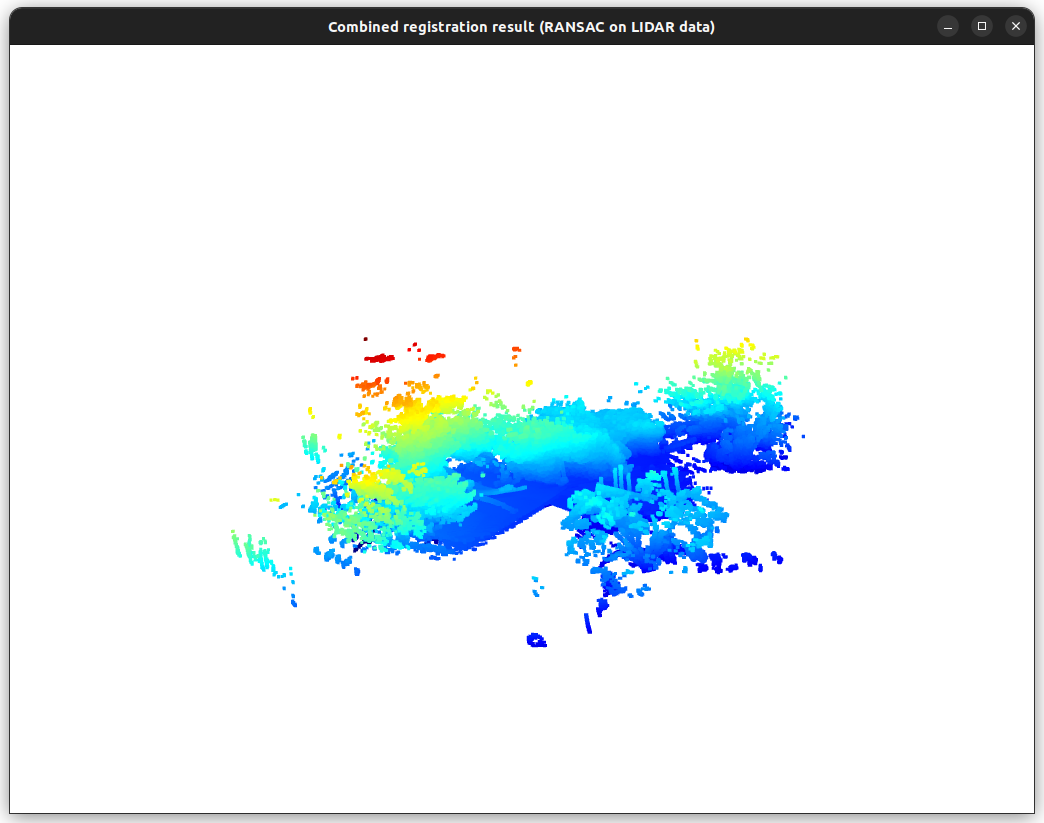
\includegraphics[width=0.7\linewidth]{RANSAC-on-LIDAR-3.png}
            \caption{\label{fig:RANSAC-on-LIDAR-3}Result fused point clouds, using RANSAC on LiDAR data.}
        \end{figure}
    \item Similarly to RANSAC results on RGBD data, we can make out a scene with several trees in the result fused point clouds here for LiDAR data. \textbf{Therefore, RANSAC performed adequately in registering LiDAR point clouds.}
\end{itemize}


\hspace{1cm}


\section*{2 - Exercise 2}

\section*{a) Step 4}

\begin{figure}[H]
    \centering
    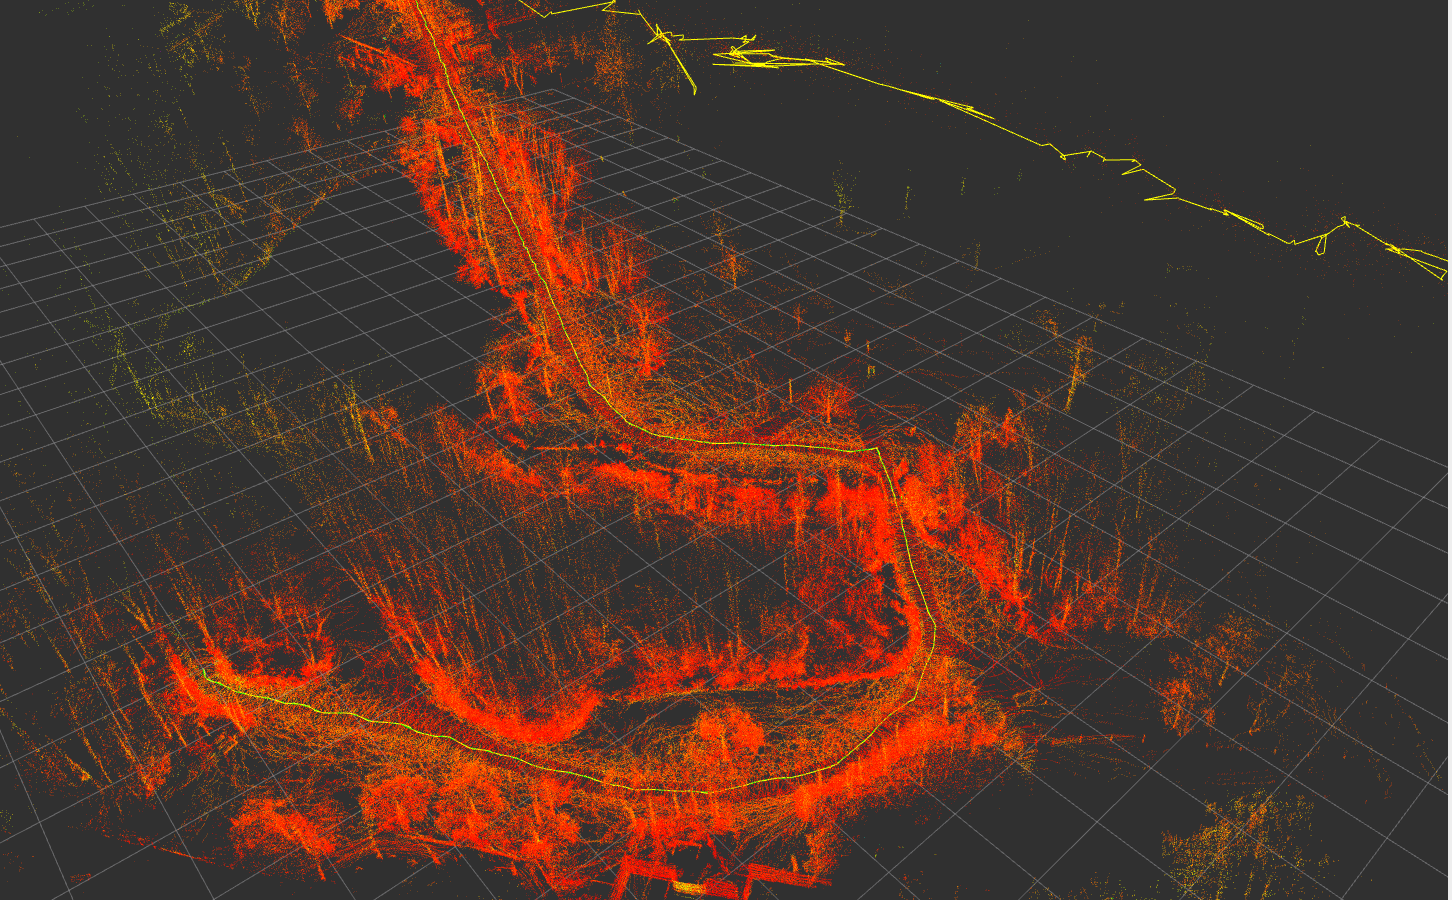
\includegraphics[width=0.7\linewidth]{LIO-SAM-park-data-2.png}
    \caption{\label{LIO-SAM-park-data-2}Result (slope area) trajectory/map of LIO-SAM algorithm on park\_dataset ROS bag.}
\end{figure}

\begin{figure}[H]
    \centering
    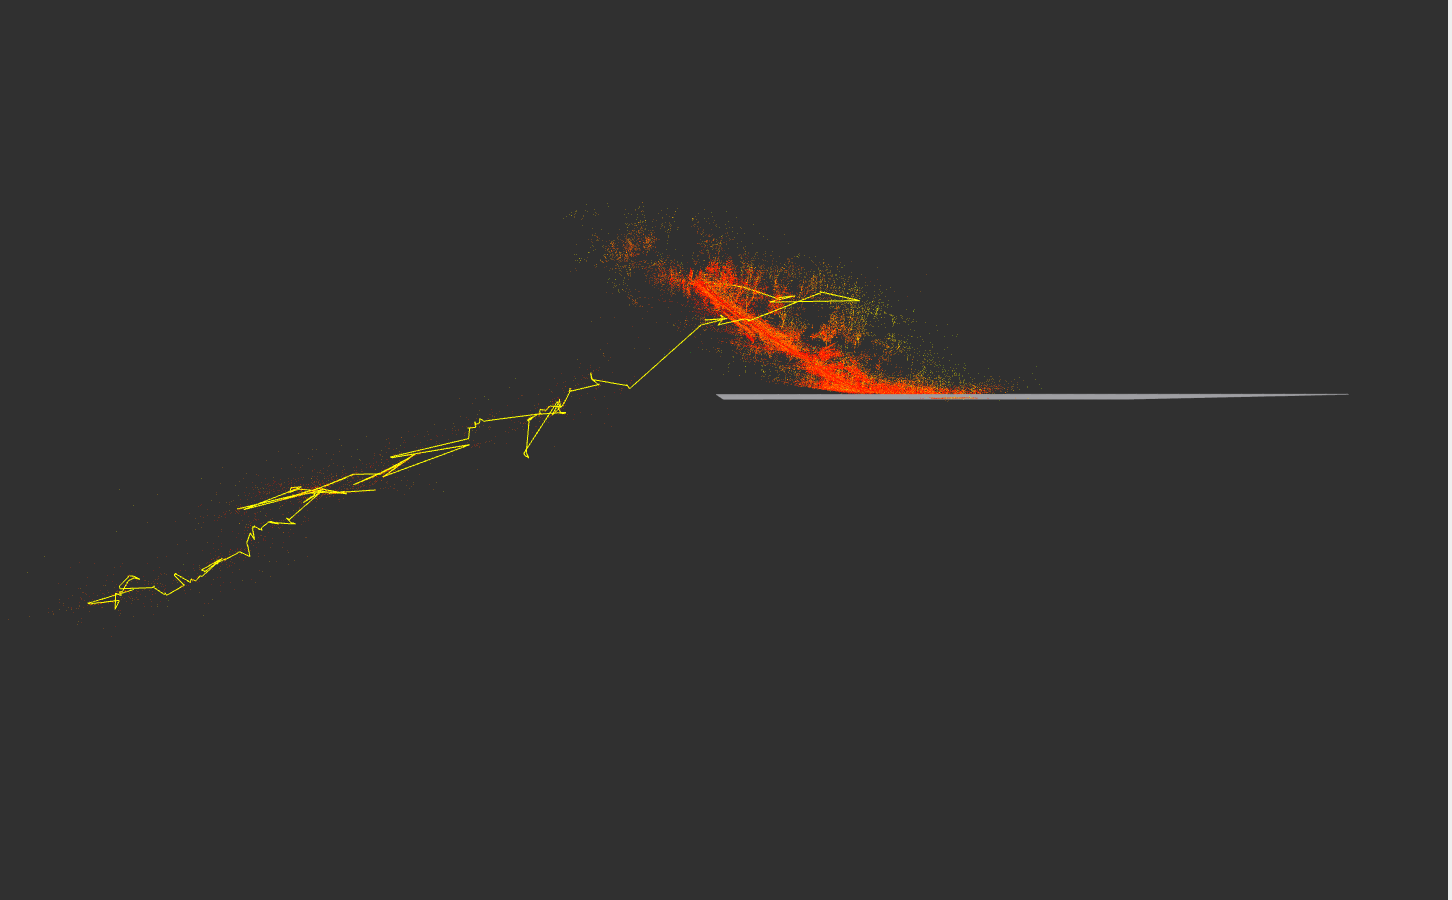
\includegraphics[width=0.7\linewidth]{LIO-SAM-park-data-4.png}
    \caption{\label{LIO-SAM-park-data-4}Result (horizontal view) trajectory/map of LIO-SAM algorithm on park\_dataset ROS bag.}
\end{figure}

\begin{figure}[H]
    \centering
    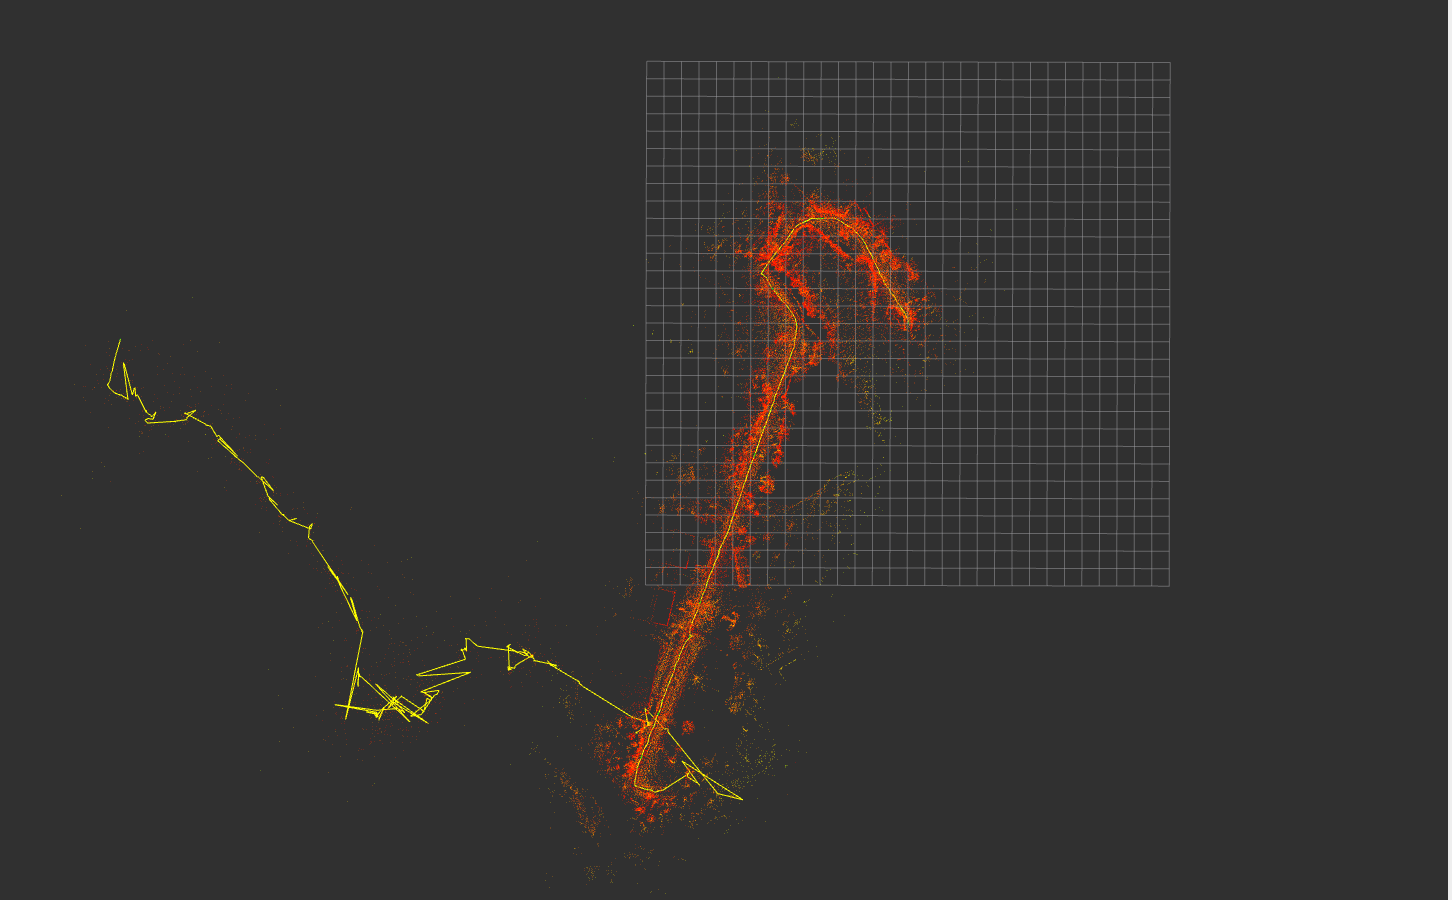
\includegraphics[width=0.7\linewidth]{LIO-SAM-park-data-6.png}
    \caption{\label{LIO-SAM-park-data-6}Result (full, top view) trajectory/map of LIO-SAM algorithm on park\_dataset ROS bag.}
\end{figure}

The zigzag path at the end signals an error. This happens as soon as the scanmatcher python program reports an error with the IMU (often a "large velocity" warning and request for IMU preintegration reset). According to some issues posted on the LIO-SAM repo by TixiaoShan, this is caused by unsynced timestamp between lidar data and IMU data. However, all the data comes from the rosbag, and this is supposed to be a working demo without changing the default settings, so we are not sure.


\hspace{1cm}


\section*{II - Homework 05}

...

\hspace{1cm}


\section*{III - Appendix}

...


\end{document}